% Intended LaTeX compiler: pdflatex
\documentclass[10pt,a4paper,UTF8]{article}
\usepackage{zclorg}
\author{emacsun}
\date{}
\title{使用 github 保存本地仓库}
\hypersetup{
 pdfauthor={emacsun},
 pdftitle={使用 github 保存本地仓库},
 pdfkeywords={},
 pdfsubject={},
 pdfcreator={Emacs 25.0.50.1 (Org mode 9.0.5)},
 pdflang={English}}
\begin{document}

\maketitle
\tableofcontents
\titlepic{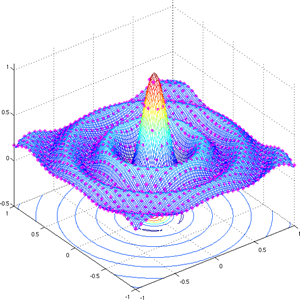
\includegraphics[scale=0.25]{../../img/sinc.PNG}}
github 是一个比较理想的 git 仓库托管地,至少我的学习笔记,平常学习的代码以及个人博客都托管到了 github 上,随时随地都可以访问得到。本文以托管我的 Emacs(当然我使用 \href{https://spacemacs.org}{spacemacs})配置为例,记录如何使用 github 托管本地仓库。



\section{首先把 .spacemacs 换成 .spacemacs.d}
\label{sec:org9d4cb68}


目前我使用 \href{http://spacemacs.org/}{spacemacs} 来配置 Emacs,配置都写在 \texttt{.spacemacs} 里,打算用 \texttt{.spacemacs.d} 文件夹来保存我的配置。

好处之一是便于版本管理。

\texttt{.spacemacs} 文件在 windows 上会被当成扩展名为 \texttt{.spacemacs} 的无名字文件, 当我要把之前的 \texttt{backup.spacemacs} 中的 \texttt{backup} 去掉时,windows 会勒令我必须键入文件名。在 \texttt{.spacemacs.d} 中 \texttt{.spacemacs} 是以 \texttt{init.el} 的形式存在的。

还有其他的好处, 见 \href{https://zilongshanren.com/}{子龙闪人} 博客中的相关叙述。岔开一句: \href{https://zilongshanren.com/}{子龙闪人}  的博客是值得收藏的价值博客。
\section{在 github 上创建一个仓库}
\label{sec:org9d1958b}


这一步简单,不会问度娘。

假设已经在 github 创建了仓库,地址是 \url{https://github.com/emacsun/.spacemacs.d}

\section{把本地仓库托管到 github 上去}
\label{sec:org93fa8f8}


进入本地文件夹 \texttt{.spacemacs.d} ,执行:
\begin{verbatim}
1. git init  // 初始化本地 git 环境
2. git config --global user.name yourname  //配置用户名,如果已经做过就可以忽略
3. git config --global user.email youremail //配置 Email
4. git add . //添加新文件
5. git commit -m "inital version"  //初始版本提交
6. git remote add origin https://github.com/emacsun/.spacemacs.d //添加远程版本库
7. git push -u origin master //将本地 master 分支提交到远程分支
\end{verbatim}

如果第一次执行第 7 步的时候,报错说:提交失败,因为远程仓库包含您本地尚不存在的提交,就把第 7 步换成

\texttt{git push -u origin master -f}

去强行提交,覆盖远程仓库原有的东西(很可能是一个 README.MD 文件)

至此结束,以后每修改一次都执行第 4,第 5 和第 7 步即可。
\section{使用 \texttt{SSH} 而不是 \texttt{https}}
\label{sec:orgfdd7e37}


为什么不用 \texttt{https} 而用 \texttt{ssh} ?

\begin{enumerate}
\item \texttt{https} 每次 \texttt{push} 都要输入账户名和密码,麻烦。
\item \texttt{ssh} 更安全,且不需要每次 \texttt{push} 都输入账户名和密码。并且据说 \texttt{ssh} 速度更快。
\end{enumerate}

如何创建公钥,并上传到 github 上,请参见\href{http://www.open-open.com/lib/view/open1416647023164.html}{这里} ,对于我来说,只需要把上一小节的第 6 步:
\begin{verbatim}
6. git remote add origin https://github.com/emacsun/.spacemacs.d //添加远程版本库
\end{verbatim}

换成:
\begin{verbatim}
6. git remote add origin git@github.com:emacsun/.spacemacs.d //添加远程版本库
\end{verbatim}
即可。如果事先已经添加了 \texttt{https} 的远程仓库,则需要:
\begin{verbatim}
git remote remove origin
git remote add origin git@github.com:emacsun/.spacemacs.d //添加远程版本库
\end{verbatim}

easy!
\end{document}
